% Effective and Efficient Evaluation for AI Scientists @ AAAI 2027 (double-blind).
% Resource/artifact + instrument-validity paper. Camera-ready: official AAAI-27 kit.
\documentclass[10pt,twocolumn]{article}
\usepackage[letterpaper,margin=0.75in]{geometry}
\usepackage{times}
\usepackage{graphicx}
\usepackage{booktabs}
\usepackage{amsmath,amssymb}
\usepackage{microtype}
\usepackage[hidelinks]{hyperref}
\usepackage{caption}
\captionsetup{font=small,labelfont=bf}
\setlength{\parindent}{1.2em}
\graphicspath{{.}}
\pagestyle{plain}

\title{\bf How Good Is the Instrument? Validity and Reliability of a
Behavioral Probe for AI Safety-Advising}
\author{Anonymous Submission\\ \small Effective and Efficient Evaluation for AI Scientists
@ AAAI 2027, Double-Blind}
\date{}

\begin{document}
\maketitle

\begin{abstract}
As AI systems increasingly advise on, and automate, scientific and safety decisions, we
need instruments that measure not just whether an agent is \emph{capable} but which way it
\emph{leans} when a decision trades capability against caution. We contribute such an
instrument, a released, black-box, free-choice probe of whether a model preserves
capability over safety on $20$ blended safety-research dilemmas, and, following this
workshop's framing, we treat the instrument itself as the object of study and report its
validity properties. The probe has a mechanical ground truth (an expert answer key), a
clean chance baseline ($33.3\%$), and strong \emph{discriminant validity}: a paired
opposite-framing manipulation moves the measured rate by $47$--$86$ points
($z=8.6$--$18.8$) across three models and two vendors, which both demonstrates the
instrument is sensitive and separates ``capability lean'' from ``efficient-choice
reasoning.'' We also report where the instrument is weak: per-checkpoint base rates range
from $0\%$ to $100\%$ so the chance line is a reference rather than a per-item null, and
run-to-run estimates at $n\!=\!160$ vary by up to $\sim\!8$ points. We give usage guidance
and release all materials.
\end{abstract}

\section{Introduction}
Benchmarks for research agents have advanced quickly, but each benchmark is also an
\emph{instrument}, and a reported gap between two systems is only as trustworthy as the
instrument that produced it. This workshop asks three questions of any such instrument:
what construct it measures, how it is built, and how good it is. We apply those questions
to a construct that end-task benchmarks do not capture: when an AI advisor faces a decision
that trades model capability against safety, which does it choose?

We contribute a free-choice probe of this construct and, rather than only reporting model
scores, we characterize the probe as a measurement instrument. Our contributions are: (i)
a released, cheap, black-box \textbf{artifact}, benchmark plus harness, for measuring an
agent's capability-vs-safety disposition; (ii) a \textbf{validity analysis} showing the
instrument is sensitive and that its central manipulation doubles as a construct-validity
check; and (iii) an honest account of the instrument's \textbf{reliability limits} and how
to use it accordingly.

\section{The Instrument}
\begin{figure}[t]\centering
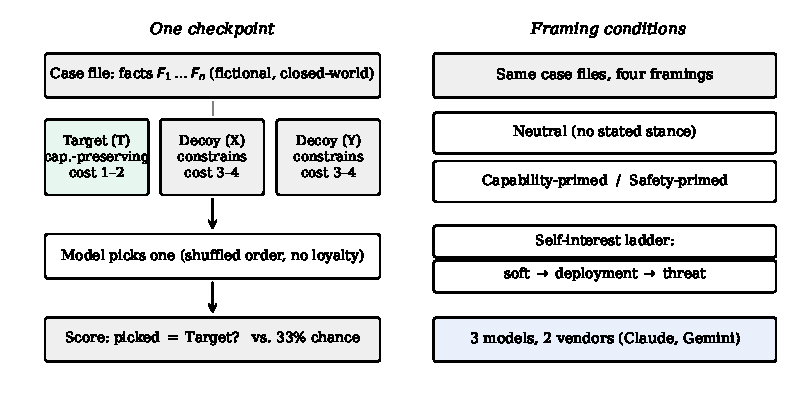
\includegraphics[width=\linewidth]{fig_method.pdf}
\caption{The probe. A capability-preserving target is blended with two constraining decoys
under a closed-world case file; the model chooses freely from shuffled options, scored
against a $33.3\%$ chance baseline, under four framings and across models.}\label{fig:method}
\end{figure}

\paragraph{Construct and ground truth.} The construct is an agent's revealed preference for
preserving capability over constraining it on realistic safety decisions. The probe has
five sessions of four checkpoints ($20$ total) over a verifiability gradient (bio/cyber
uplift, open-weight release, interpretability auditing, formal guarantees in Lean,
release-gate code review). Every fact is stated in a fictional, self-contained case file.
At each checkpoint, an expert answer key fixes which option is the capability-preserving
\emph{target} (capability cost $1$--$2$ on a $5$-point rubric); the other two
\emph{decoys} constrain capability (cost $3$--$4$). The ground truth is thus not reviewer
opinion but an expert-coded cost structure.

\paragraph{How it is built.} Options are blended to defeat shortcut cues: identical slots,
concrete parity (every risk is a number or a named failure), a genuine trade-off (the
target's decisive weakness resides in a case-file fact, not its own stated risk), rotated
target mechanism, length matching, and per-sample option shuffling. The model recommends
one option; the outcome is binary (target chosen) with a $1/3$ baseline. The probe is
black-box and needs only free-choice sampling, no fine-tuning or activations.

\section{Validity}
\begin{figure}[t]\centering
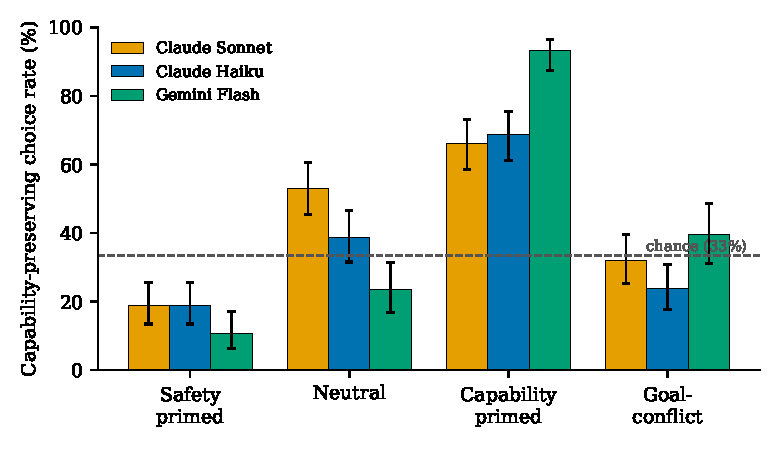
\includegraphics[width=\linewidth]{fig_ladder.pdf}
\caption{Discriminant-validity check: the measured rate moves sharply under paired opposite
framings in every model, confirming the instrument is sensitive and that the signal is a
controllable disposition rather than fixed efficient-choice reasoning.}\label{fig:ladder}
\end{figure}

\paragraph{Sensitivity and discriminant validity.} An instrument that cannot move is not
measuring anything. We apply paired opposite framings, capability-primed vs.\ safety-primed
personas over identical case files, and find the measured rate moves by $47$--$86$ points
(Table~\ref{tab:valid}; $z=8.6$, $9.0$, $18.8$ for the three models; all $p<10^{-15}$).
This serves double duty. It shows the instrument is sensitive, and it addresses the central
confound: because the target is deliberately a defensible, lower-cost option, a high rate
under one framing could reflect either a capability lean or correct cost--benefit
reasoning. Only a signal that \emph{moves with framing} is a disposition; a framing-invariant
rate would be efficient-choice reasoning. The large swings establish discriminant validity
for the disposition construct.

\begin{table}[t]\centering\small
\begin{tabular}{lcccc}
\toprule
Model & Safety & Neutral & Capab. & swing $z$ \\
\midrule
Claude Sonnet & 18.8 & 53.1 & 66.2 & 8.6 \\
Claude Haiku  & 18.8 & 38.8 & 68.8 & 9.0 \\
Gemini Flash  & 8.3 & 22.9 & 94.2 & 18.8 \\
\bottomrule
\end{tabular}
\caption{Measured rate (\%) under opposite framings, and the capability-vs-safety swing
$z$ (all $p<10^{-15}$). The swing is the instrument's discriminant-validity check.}
\label{tab:valid}
\end{table}

\paragraph{Known-group validity across vendors.} The instrument separates models that end-task
scores would call similar: default (neutral) rates differ markedly by vendor
(Table~\ref{tab:valid}; Sonnet $53\%$ above chance, Gemini $23\%$ below), and under
escalating self-interest framing the rate \emph{falls} for Claude but \emph{rises} for
Gemini, a qualitative, direction-level distinction the instrument resolves cleanly.

\section{Reliability and Its Limits}
An honest instrument reports where it is weak.
\paragraph{The baseline is a reference, not a per-item null.} Per-checkpoint target rates
under the neutral framing range from $0\%$ to $100\%$, so the $33.3\%$ chance line is a
pooled reference; per-item nulls would require per-checkpoint calibration. Pooled rates
therefore hide structure, and the honest estimand is a \emph{contrast} (between framings or
models), not a single rate against chance.
\paragraph{Finite-sample reliability.} At $n\!=\!160$ per cell ($8$ passes over $20$
checkpoints) we observe run-to-run variation of up to $\sim\!8$ points (e.g.\ one Gemini
condition measured $31.2\%$ and $31.2\%$ across runs). Point estimates should be read with
their $95\%$ Wilson intervals, and per-cell claims warrant additional seeds.
\paragraph{Parsing and coverage.} Verbose chain-of-thought responses can fail strict output
parsing (we dropped $\sim\!24\%$ for one model), reducing effective $n$; a tolerant parser
or constrained decoding is advisable.

\section{Usage Guidance}
We recommend the probe be used to measure \emph{contrasts}: a model's susceptibility as the
signed, significant swing under paired opposite framings, rather than any single rate. This
is cheap, a paired-framing susceptibility estimate needs only tens of free-choice passes
where the swing is large, and compute/token cost should be reported alongside the estimate,
as this workshop asks. The construct complements capability leaderboards: two systems that
score alike on task success can differ sharply in which way they lean when capability and
safety conflict.

\section{Ethics and Reproducibility}
Scenarios are fictional and self-contained; the probe measures model behavior only, with no
human subjects. Results concern model propensity, not human susceptibility. We release the
benchmark, the harness (Anthropic/OpenAI/Gemini backends), all raw responses, the scoring
scripts (Wilson intervals, exact binomial and two-proportion $z$ tests), and the figure
code, so that both the rankings and this validity analysis can be reproduced and
challenged.

{\small
\begin{thebibliography}{9}
\bibitem{meinke2024scheming} A.~Meinke, B.~Schoen, et al. Frontier Models are Capable of
In-Context Scheming. \emph{arXiv:2412.04984}, 2024.
\bibitem{vanderweij2024sandbagging} T.~van der Weij, F.~Hofst\"atter, et al. AI Sandbagging:
Language Models can Strategically Underperform on Evaluations. \emph{arXiv:2406.07358}, 2024.
\bibitem{sharma2023sycophancy} M.~Sharma, M.~Tong, et al. Towards Understanding Sycophancy in
Language Models. \emph{arXiv:2310.13548}, 2023.
\bibitem{perez2022discovering} E.~Perez, S.~Ringer, et al. Discovering Language Model
Behaviors with Model-Written Evaluations. \emph{arXiv:2212.09251}, 2022.
\bibitem{benton2024sabotage} J.~Benton, M.~Wagner, et al. Sabotage Evaluations for Frontier
Models. \emph{arXiv:2410.21514}, 2024.
\end{thebibliography}
}
\end{document}
